\section{Applying Optimizations to SGEMM\jled{Optimizing SGEMM}}
\label{sec:optimization}


The demystified GPU microarchitecture features provide a larger tuning space for computational kernels \jled{most kernels are performance-critical, right? :-)}.g
We applyg
a series of incremental optimizations to improve SGEMM performance on Kepler architecture. The optimization strategiesg
go through architectural hierarchy from CUDA core and register to memory. All the optimization strategies are inspired by the observations from our benchmarking.
\begin{itemize}
\item At core level, we orchestrate {\tt FFMA} instruction executions with a more efficient instruction scheduling set by the proper control code.
% with respect to the proper control code pattern.
\item At register level, we meticulously map operands to registers so that bank conflicts are avoided for the inner loop in Algorithm~\ref{gemm}.
\item At memory level, we select appropriate shared memory load/store width and global memory data path to mitigateg
latencies.
\end{itemize}

\subsection{Instruction Scheduling}
\subsubsection{Schedule {\tt FFMA} Instructions}
It's unrealistic to keep warp schedulers dual issue the same kinds of arithmetic instructions (i.e., {\tt FFMA}) allg
the time. Because on Kepler architecture, each warp is assigned $32$ cores privately, $4$ warp schedulers will consumeg
$128$ cores. The reminding $192-128=64$ cores are divided into $2$ 32-core groups, each $32$ coresg
are shared by $2$ warp schedulers. Two warp schedulers must negotiate who will use the extra $32$ shared cores to avoidg
resource conflict.
As noted in {\em observation 3}, the best pattern of {\tt FFMA} instructions block is a sequence of $1$ single issue(1g
{\tt FFMA}), 2 dual issues (4 {\tt FFMA}s) and 1 single issues ((1 {\tt FFMA})). As shown ing
Figure~\ref{fig:assemblycode}, the instructions in lines 3-4 and lines 6-7 are dual issued separately.g
The other two instructions in line 8 and line 11 are two single issues in terms of floating-point instructiong
execution.g
As a comparison, most of the {\tt FFMA}s are single issued in the CUDA compiler generated codes.

\begin{figure*}[htbp]
\begin{center}
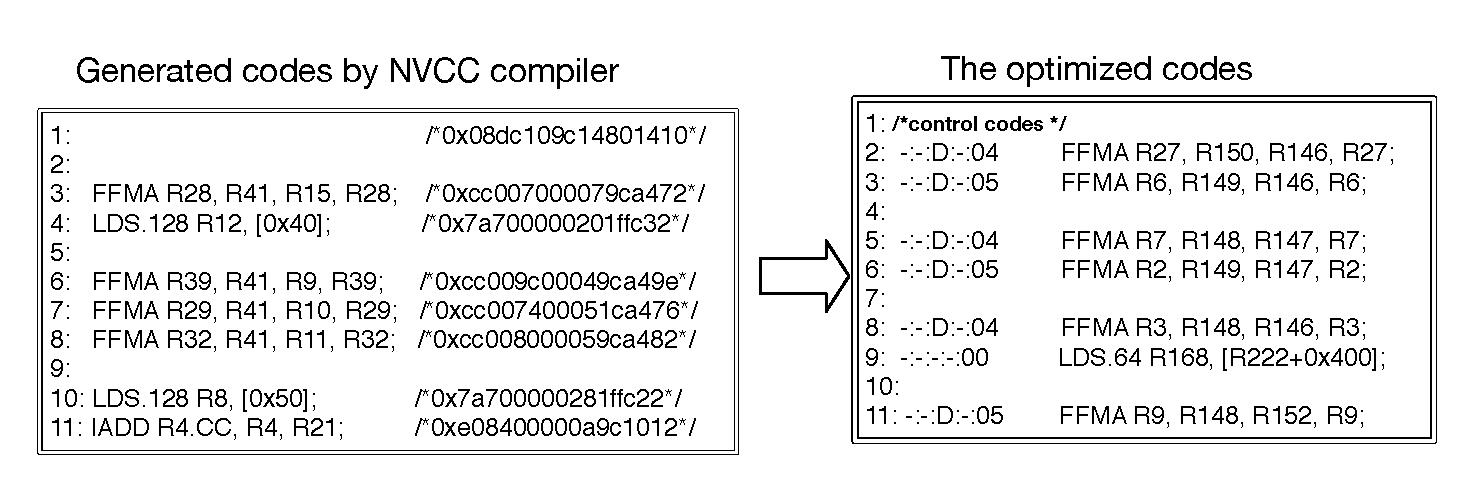
\includegraphics[scale=0.6]{assemlycode}
    \caption{The comparison of compiler generated codes and our tuned assembly codes.}
\label{fig:assemblycode}
\end{center}
\end{figure*}

\begin{figure}[htbp]
\begin{center}
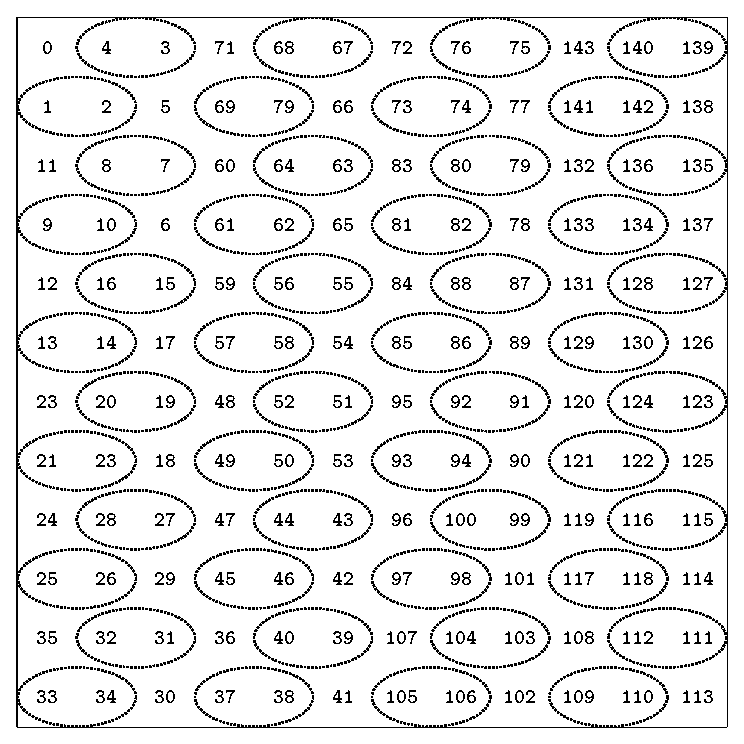
\includegraphics[scale=0.5]{order}
\caption{{\tt FFMA}s instruction scheduling to compute a $12\times 12$ sub-block of matrix C.  The numbers ing
cells denote {\tt FFMA} execution order. Dashed ellipses across two cells mean that two {\tt FFMA} instructions are dual issued in one clock cycle.}
\label{fig:order}
\end{center}
\end{figure}

By extending the basic {\tt FFMA} $7$-instruction block (section~\ref{sec:benchmark}), we depict the scheduling pattern of computing a $12\times 12$ sub-block of matrix C in Figure~\ref{fig:order}.
% illustrates the order of $144$ {\tt FFMA}s instruction execution for calculating a $12\times 12$ subblock of matrix C.
For example, the {\tt FFMA} to calculate $c_{00}$ is issued first.g
Then, two {\tt FFMA}s to
compute $c_{10}$ and $c_{11}$ are simultaneously issued. We arrange all the {\tt FFMA} instructions of SGEMM according to the order in Figure~\ref{fig:order}.

Another advantage of this execution order is less register pressure due to register reuse, which can facilitate
operand collector mechanism~\cite{collector}. Operand collector is a storage element coupled with register file and
provides inputs to the data path of the processor core for executing an instruction. \jled{This is not the first occurrence of Operand collector.} Operands may be cached and reused
in the subsequent instructions.g
The assembly code in Figure~\ref{fig:assemblycode} lists the instructions to calculate $C_{32},C_{22}, C_{21}, C_{30},g
C_{31}, C_{20}$, corresponding to the orders of $6,7,8,9,10,11$ in Figure~\ref{fig:reg}.g
With the elaborately designed computing order and register allocation, the reuse happens as follows. The {\tt FFMA} ing
Line $3$ uses cached operand {\tt R150} of line $2$, Line $3$ and Line $4$ share {\tt R146}. Thus, in dual issue modeg
{\tt FFMA} of Line $3$ and $4$ need to read 4 registers {\tt R146}, {\tt R27}, {\tt R149}, {\tt R6} instead of $6$g
registers. The corresponding bank of these registers are $0,1,3,2$ based on Table~\ref{tab:reg}, so no bank conflicts happen.
Similarly, Line 7 uses the cached operand {\tt R149} from the Line 4. In dual issue mode, two {\tt FFMAs} of Line 6 andg
Line 7 need to read $4$ registers {\tt R148}, {\tt R147}, {\tt R7} and {\tt R2}.

\begin{table}[!t]
\caption{The position table of {\tt Non-FFMA} instructions. The inner-loop is unrolled by 4 times. The first columng
records slot numbers and the first row represents iteration number.}
\label{tab:position}
\captionsetup{font=scriptsize}
\centering
\scalebox{0.78} {
\begin{tabular}{|c|c|c|c|c|}
\hline
\diagbox[width=4em, height=3em]{slot}{unroll} & 0 &1 &2 &3 \\
    \hline
    5 & ISET P0 & IADD A0 & & XOR smB \\
    \hline
    11 & LDS.64 smA & LDS.64 smA & LDS.64 smA & LDS.64 smA \\
    \hline
    17 & LDS.64 smA & LDS.64 smA & LDS.64 smA & LDS.64 smA \\
    \hline
    23 & LDS.64 smA & LDS.64 smA & LDS.64 smA & LDS.64 smA \\
    \hline
    29 & LDS.64 smA & LDS.64 smA & LDS.64 smA & LDS.64 smA \\
    \hline
    35& IADD K, -4 & IADD A1 & TEXDEPBAR & \\
    \hline
    41 & LDS.64 smB & LDS.64 smB & LDS.64 smB & LDS.64 smB \\
    \hline
    47 & LDS.64 smB & LDS.64 smB & LDS.64 smB & LDS.64 smB \\
    \hline
    53 & LDS.64 smB & LDS.64 smB & LDS.64 smB & LDS.64 smB \\
    \hline
    59 & LDS.64 smB & LDS.64 smB & LDS.64 smB & LDS.64 smB \\
    \hline
    65 & & &STS.64 writeS & ISETP P2 \\
    \hline
    71 & & & & \\
    \hline
    77 & & IADD B0 & & LDG A \\
    \hline
    83 & LDS.64 smA & LDS.64 smA & LDS.64 smA & LDS.64 smA \\
    \hline
    89 &ISETP P3 & & &\\
    \hline
    95 & LDS.64 smA & LDS.64 smA & LDS.64 smA & LDS.64 smA \\
    \hline
    101 & & & STS.64 loadB0 & LDG B \\
    \hline
    107 & & & STS.64 loadB2 & XOR writeS \\
    \hline
    113 & & & & \\
    \hline
    119 & LDS.64 smB & LDS.64 smB & LDS.64 smB & LDS.64 smB \\
    \hline
    125 & & & XOR smA & \\
    \hline
    131 & LDS.64 smB & LDS.64 smB & LDS.64 smB & LDS.64 smB \\
    \hline
    137 & & & & \\
    \hline
    143 & & IADD B1 & BAR.SYNC & BAR Loop \\
    \hline
\end{tabular}
}

\end{table}

\subsubsection{Schedule {\tt non-FFMA} Instructions}

After setting the order of {\tt FFMA}, other {\tt non-FFMA} instructions should be inserted in proper positions tog
assure the correct program without losing performance. In order to tolerate instruction latency, the
distance of dependent instructions needs to be larger than their latency. The distance is approximated as
\begin{equation}
\label{eq:inst}
distance = \frac{4\times\#instructions}{7}.
\end{equation}
A $7$-instruction scheduling block costs $4$ clock cycles to be issued in dual issue mode.g
Therefore, if we assume two interleave instructions have a distance $L$, at least $\frac{L*7}{4}$ instructions are needed.g
% two instructions of $L$ distance, then $\frac{L*7}{4}$ instructions are needed.g
Besides, the remained number of slotsg
to insert these instructions is estimated as

\begin{displaymath}
\#slots = \frac{rx\times ry\times bk}{ffmas\_in\_schedule\_block}=\frac{12\times 12\times 4}{6}=24\times 4.
\end{displaymath}
$rx\times ry\times bk$ yields the total number of {\tt FFMA}s for one thread inside register blocking loop in Algorithm~\ref{gemm}, where $rx$ and $ry$ are register blocking size and $bk$ is the unrolling factor.
$ffmas\_in\_schedule\_block$ is the number of {\tt FFMA} instructions inside one scheduling block, which is $6$ by our $1-2-2-1$ dual issue pattern in section~\ref{sec:benchmark}.
According to these principles, we first arrange {\tt LDS}, {\tt STS}, {\tt LDG} because of their long latencies. The
schedule slots are illustrated in two dimension in Table~\ref{tab:position}.
Note that we use double buffers to hide the latency of {\tt LDG} from global memory, which is $200$ clock cycles.
Every $4$ loops require $2$ {\tt LDG}s to load data from global memory to registers, $4$ {\tt STS}s to store data fromg
registers to shared memory. A read after write (RAW) dependency exists between {\tt
LDG} and {\tt STS}.g
From equation~\ref{eq:inst}, $\frac{200\times 7}{4} = 350$ instructions are needed between them.
We put {\tt LDG} and  {\tt STS} in position $P[77][3]$ and $P[65][2]$ respectively in Table~\ref{tab:position}.g
Thus, $143-77 + 144\times 2 + 65=419$ ($>350$) instructions are between them, which is enough to hide latency of {\tt LDG}s.
% resulting in a distance of $\frac{4\times 419}{7}=239$ clocks,.

The arrangement of {\tt LDS}s, loading data from shared memory for double buffers of $A$ and $B$, follows the same approach with {\tt LDG}s.
A {\tt LDS} has a latency of $40$ clock cycles, thus $\frac{40\times 7}{4}=70$ instructions are needed to interleave {\tt LDS} and {\tt FFMA}.g
In Table~\ref{tab:position}, {\tt LDS} in $P[11][3]$ reads data from {\tt STS} in $P[65][2]$,g
the distance between them is more than $40$ clock cycles.g
At the end, a {\tt BAR.SYNC} is inserted after {\tt STS} but before {\tt LDS} to make sure that data in shared memory is ready.g
Other instructions such as {\tt XOR}, {\tt IADD}, {\tt ISETP} are inserted according to data dependency, they doesn't influence the performance because of their short latencies.


\subsection{Register Allocation}

To allocate registers for $A$ column, $B$ row and $C$ sub-matrix as Algorithm~\ref{gemm}, we have three objectives: correctness, no bank conflict and tight register indices.
{\tt LDG.128} restricts $4$ words alignment for registers.
Since NVIDIA GPU does not have $128$-bit register, a $128$-bit load instruction ({\tt LDG.128}) writes the data to four consecutive $32$-bit registers {\tt RN}, {\tt RN+1}, {\tt RN+2}, and {\tt RN+3} given one destination register $RN$.
% in order to use $128$-bit load, one destination register $RN$ is given,g
% results will be written to
% four $32$-bit registers: {\tt RN}, {\tt RN+1}, {\tt RN+2}, {\tt RN+3}.g
We discover an undocumented restriction that $N\%4=0$ to avoid illegal instruction error.
% It's not hard to understand this restriction,g
The $4$ words alignment restriction for {\tt LDG.128} simplifies hardware logic and cuts down power.
Since we use {\tt LDG.128} to load $A$ and $B$, there are $2$ bank allocation choices limited by $N\%4==0$ restriction and Kepler's bank distribution (Table~\ref{tab:reg}).g
We assume allocate $A$ matrix bank $\begin{bmatrix} 0 \\ 1  \end{bmatrix}$,
    $B$ bank $\begin{bmatrix} 2 & 3 \end{bmatrix}$ as shown in Figure~\ref{fig:reg}, 2 choices left for $C$,g
$\begin{bmatrix} 1 & 2 \\ 3 & 0  \end{bmatrix}$ andg
$\begin{bmatrix} 3 & 1 \\ 0 & 2  \end{bmatrix}$.
The $4=2\times2$ bank patterns for SGEMM are equivalent in performance, then we arbitrarilyg
choose $\begin{bmatrix} 0 \\ 1  \end{bmatrix}$ $\begin{bmatrix} 2 & 3 \end{bmatrix}$
    $\begin{bmatrix} 1 & 2 \\ 3 & 0  \end{bmatrix}$ for $A$, $B$ and $C$ respectively.
We use different colors to represent the four banks and show the bank allocation when computing a $12 \times 12$ sub-matrix of C in Figure~\ref{fig:reg}.
% We have $2\times2$ bank patterns for SGEMM, these four patterns are equivalent in performance,
To allocate actual register index, we choose continuous register index so that register index do not get too big to exceed 255 restriction. \jled{Is the left sentence necessary?}
We can verify that every $C_{ij}$, $A_i$ and $B_j$ have different banks in Figure~\ref{fig:reg}, thus register bank conflicts are successfully avoided.
% for example $C_{01}$'s color is white, $A_0$'s color is green and $B_1$'s color is red, .

\begin{figure}[htbp]
\begin{center}
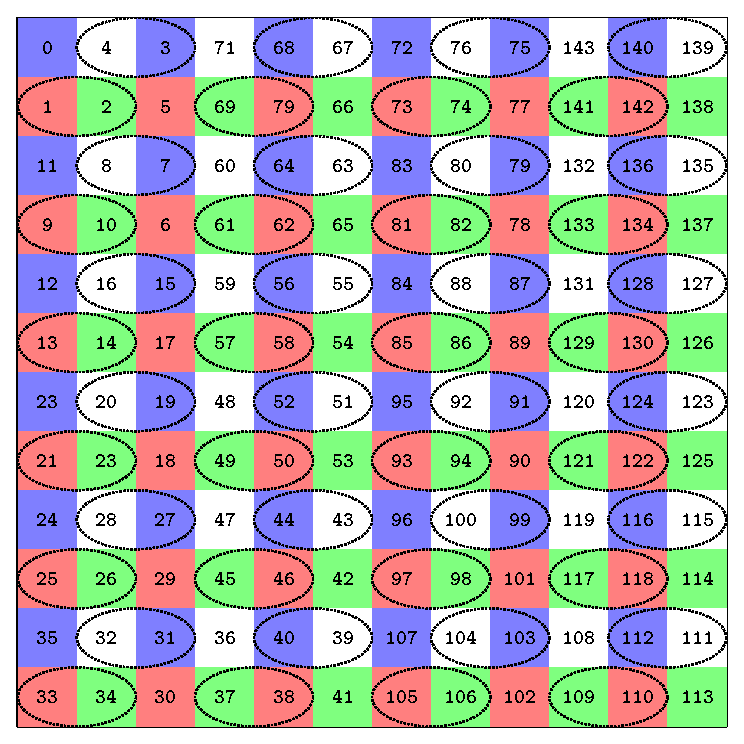
\includegraphics[scale=0.5]{reg}
\caption{An illustration of register bank allocation. The number in the cell is register number.
    The leftmost column registers are allocated to one block-column of $A$, the
topmost row registers are allocated to one block-row of $B$, and the others are registers for
a $12 \times 12$ sub-matrix $C$. Different colors denote the mapping of register banks as in Table~\ref{tab:ref}: green$\rightarrow$bank0,g
blue$\rightarrow$bank1, gray$\rightarrow$bank2, red$\rightarrow$bank3.}
\label{fig:reg}
\end{center}
\end{figure}


\subsection{Memory Movement}
% According to the optimization observation on memory access suggested by microbenchmark,g
According to our benchmarking observations, we use {\tt LDG.128} to load data from global memory through texture cache
and {\tt LDS.64} to load data from shared memory.g
We also have additional reasons to adopt them in SGEMM kernel.g
First, using {\tt LDG.128} reduces load instructions, hence reduce {\tt non-FFMA}s. %\jled{use load instead of non-FFMA. Use non-FFMA seems complicated.}g
In the inner loop of Algorithm~\ref{gemm}, we need three {\tt LDG.128} instead of twelve {\tt LDS.32} to read twelve
words from $A$ column.
Second, the shared memory transaction size is 256 bytes, which forces each request being split into multiple transactions.
% it is another story for shared memory.g
If we use {\tt LDS.128}, we can not infer the time of the second transaction by inspecting the inner loop, so it is
difficult to eliminate potential bank conflicts between {\tt LDS.128}s and {\tt FFMA}s..g
However, it's determinable for {\tt LDS.64}, since a transaction just happens two cycles after the instruction is
issued. \jled{don't understand this sentence.}


